% !TeX root = 191121.tex
\begin{frame}[t]{Домашнее задание: задача}
Как удобно писать Telegram-ботов?

Требования:
\begin{itemize}
\item Можно писать бота и не думать о Telegram Bot API.
\item Можно тестировать автоматически.
\item Можно тестировать бота отдельно от логики игры.
\end{itemize}
\end{frame}

\begin{frame}[t]{Архитектура-1}
\begin{center}
	\includegraphics[width=\textwidth]{general-bot-arch.pdf}
\end{center}
\end{frame}

\begin{frame}[t]{Связность и зацепление}
\begin{center}
	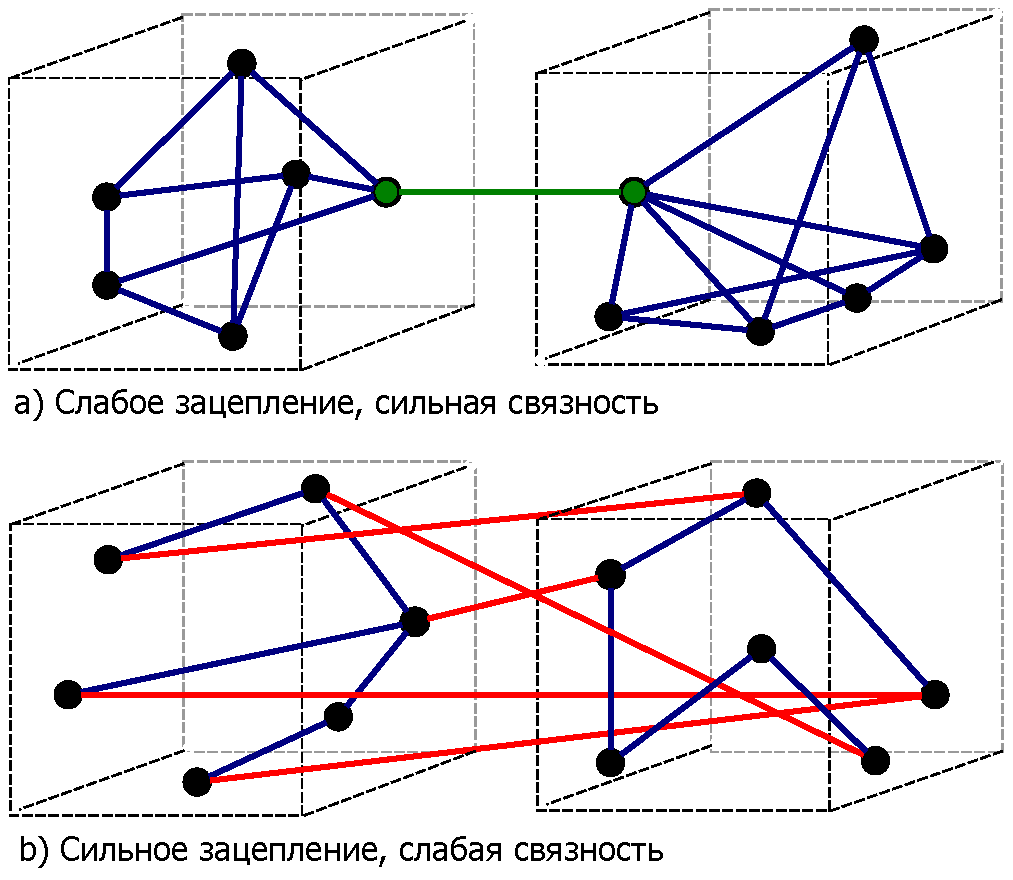
\includegraphics[height=0.8\textheight]{CouplingVsCohesion.pdf}
\end{center}
\end{frame}

\begin{frame}[t]{Архитектура-2}
\begin{center}
	\includegraphics[width=\textwidth]{user-independent-bot-arch.pdf}
\end{center}
\end{frame}

\begin{frame}[t]{Чего добились}
\begin{itemize}
	\item Можно написать $N$ способов запуска бота и $M$ ботов за $\mathcal O(N+M)$ кода.
	\item В частности, один из способов запуска "--- автоматические тесты.
	\item Из-за \texttt{UserIndependentBot} в боте нельзя послать сообщение не тому пользователю.
	\item В процедурном стиле пришлось бы протаскивать много-много параметров.
\end{itemize}
\end{frame}
